\documentclass{beamer}
\usepackage{preamble_beamer}


\title[Случайные процессы]{Лекция 2. Случайные процессы в непрерывном времени} % The short title appears at the bottom of every slide, the full title is only on the title page


\begin{document}

\begin{frame}
\titlepage 
\end{frame}

\begin{frame}{Рекап прошлой лекции}
    \begin{itemize}
        \item УМО относительно $\sigma$-алгебры и с.в.: определение, основные свойства
        \item Случайный процесс -- совокупность с.в., проиндексированных временем
        \item Фильтрация -- последовательность вложенных $\sigma$-алгебр, формализуют поток информации, доступный к моменту t
        \item Мартингал -- $\E \left[ X_{t+1} | \F_t\right] = X_t$. "Непредсказуемый" процесс. Случайное блуждание как пример мартингала.
        \item Дискретный стохастический интеграл -- PnL торговой стратегии. 
        \item Теорема Дуба об остановке: $\E X_{\tau} = \E X_0$
    \end{itemize}
\end{frame}

%%\section{Броуновское движение}

\begin{frame}{Случайные процессы}
    Пусть $(\Omega, F, \mathbb{P})$ -- вероятностное пространство.
    \begin{block}{Определение}
    Случайный процесс -- набор случайных величин $\xi_t, t \in [0, T]$ заданных на одном и том же вероятностном пространстве.     
    \end{block}
    
    \begin{block}{Конечномерные распределения}
        Всевозможные совместные распределения с.в. $\xi_{t_1}, \ldots, \xi_{t_n}$ называются конечномерными распределениями процесса $\xi_t$:
        $$
            F_{t_1, \ldots, t_n} (x_1, \ldots, x_n) = \mathbb{P}(\xi_{t_1} \leq x_1, \ldots, \xi_{t_n} \leq x_n)
        $$
    \end{block}

    \begin{itemize}
        \item Случайный процесс -- функция двух переменных $\xi_t = \xi(t, \omega)$, измеримая по второму аргумету $\forall t$.
        \item Отображение $t : \xi_t(\omega)$ при фиксированном $\omega$ -- траектория(реализация) процесса.
    \end{itemize}
\end{frame}

\begin{frame}{Примеры случайных процессов}
    Пусть $\mathcal{T}=[0,1]$, $\eta \sim N(0,1)$. Положим $\xi_t = t \cdot \eta$.
    Свойства:
    \begin{itemize}
        \item $\E \xi_t = 0$
        \item $\mathrm{Var} \xi_t = t^2$
        \item $cov(\xi_t, \xi_s) = ts$
    \end{itemize}
    
    % \begin{figure}[ht]
    % \centering
    % 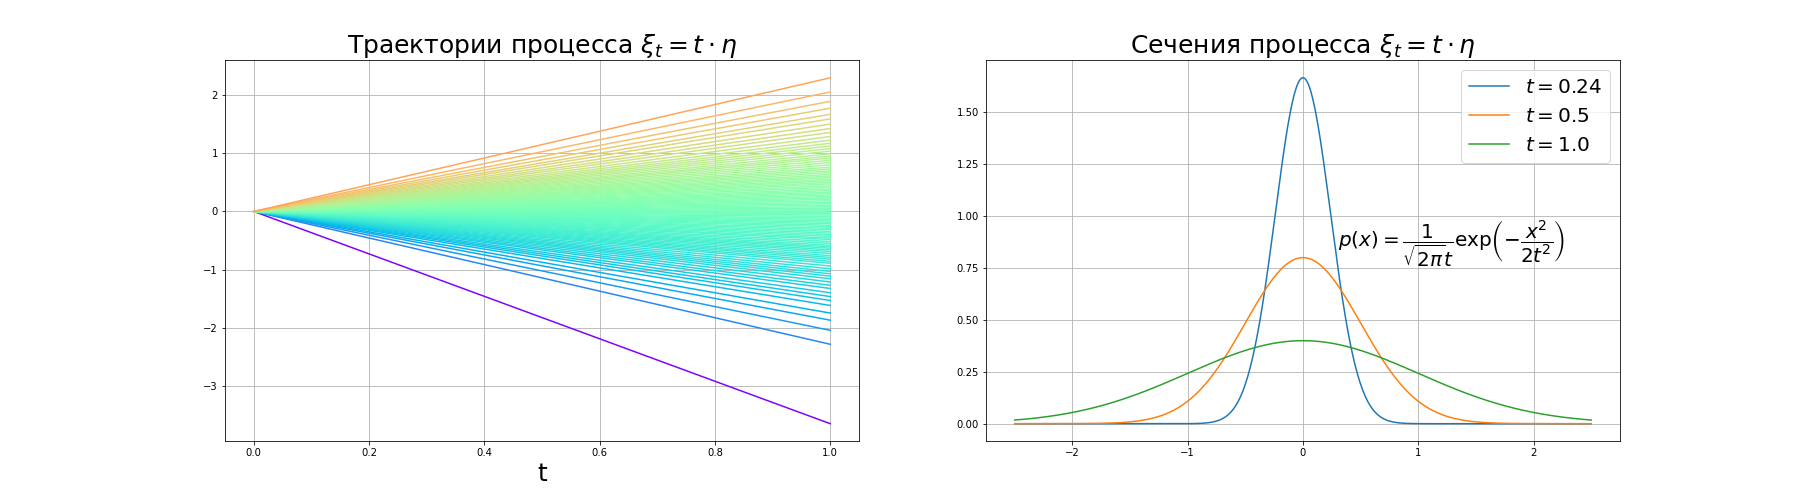
\includegraphics[width=1.2\textwidth]{1_figs/process_example_1.png}
    % \end{figure}

    \noindent\makebox[\textwidth]{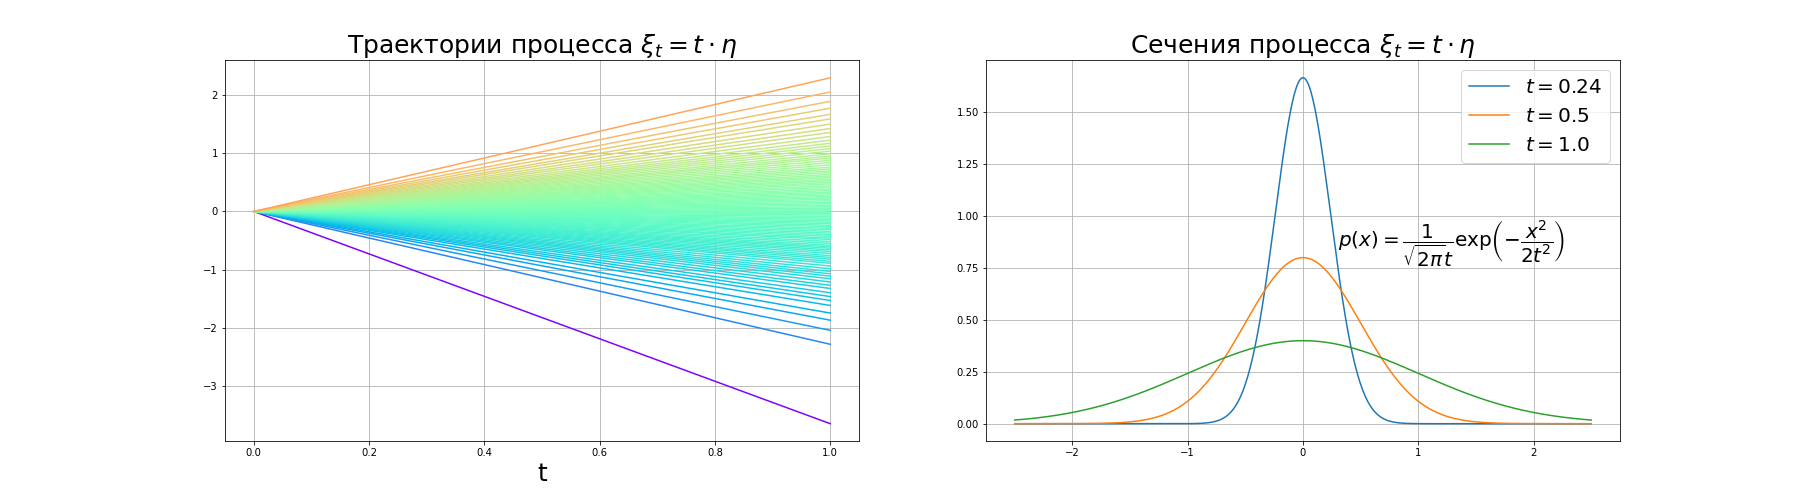
\includegraphics[width=1.2\textwidth]{1_figs/process_example_1.png}}
\end{frame}

\begin{frame}{Примеры случайных процессов}

    Пусть $\mathcal{T}=\mathbb{N}$, $\xi_t \sim Be(1/2)$ -- i.i.d.
    $$X_t = \sum_{s=1}^{t} \xi_s$$     
    Свойства:
    \begin{itemize}
        \item $\mathbb{E} X_t = 0, \; \mathrm{Var} X_t = t$
        \item $\mathbb{E} \left[ X_t | X_{t-1} \right] = X_{t-1}$
        \item $\mathrm{cov}(X_t, X_s) = \min(t, s)$
        \item Приращения $X_t - X_s \sim Binom(t-s, 0.5)$, независимы.
    \end{itemize}

    \makebox[\textwidth]{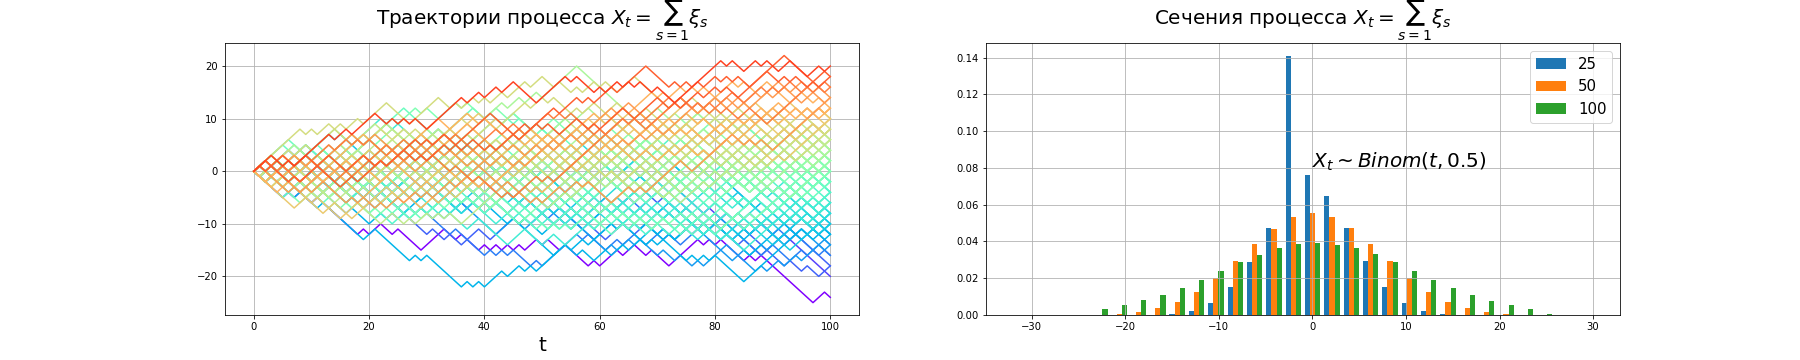
\includegraphics[width=1.2\textwidth]{1_figs/process_example_2.png}}
\end{frame}

\begin{frame}{Предел случайного блуждания}
    Пусть $X_k$ -- случайное блуждание. Введём процесс с непрерывным временем:
    $$
        B_{n}(t) = \frac{1}{\sqrt{n}} X_{\lfloor n \cdot t \rfloor}
    $$
    \begin{itemize}
        \item $\E B_n(t) = 0, \; \mathrm{Var} B_n(t) = \dfrac{\lfloor n \cdot t \rfloor}{n} \approx t$
        \item $B_t - W_s \sim \frac{1}{\sqrt{n}} Binom(t-s, 0.5) \to N(0, t-s)$ при $n\to\infty$.
    \end{itemize}
    \makebox[\textwidth]{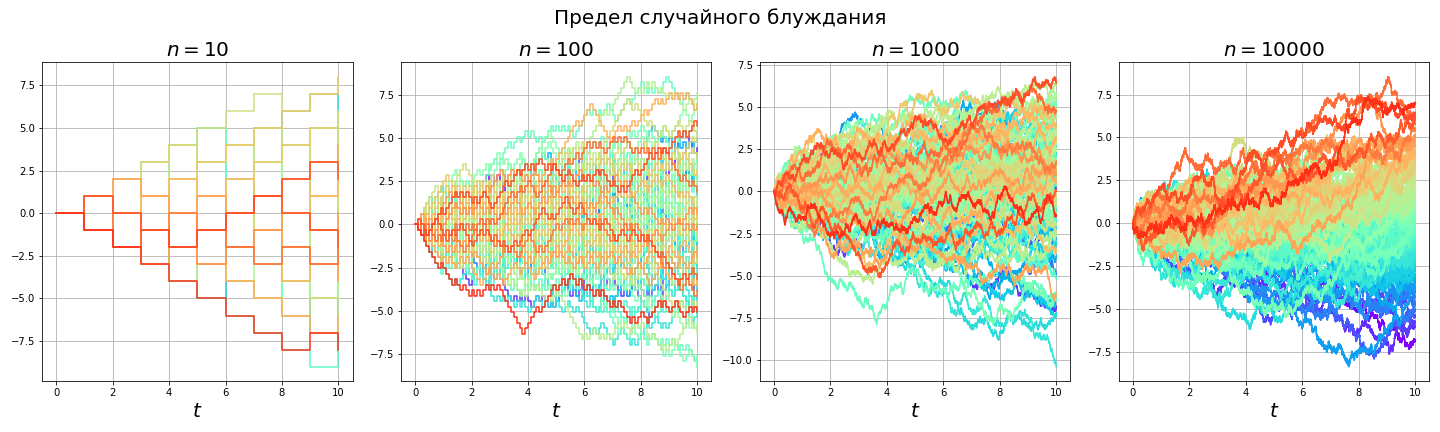
\includegraphics[width=1.2\textwidth]{2_figs/random_walk_limit.png}}
\end{frame}

\begin{frame}{Броуновское движение}
    \begin{block}{Определение}
        Случайный процесс $B_t$ называется броуновским движением (винеровским процессом), если:
        \begin{itemize}
            \item $B_0 = 0$
            \item $\forall s < t: \; B_t - B_s \sim N(0, t - s)$
            \item $\forall s_1 < t_1 \leq s_2 < t_2$ приращения
            $B_{t_2} - B_{s_2}, B_{t_1} - B_{s_1}$ -- независимы
            \item Траектории $B_t$ почти наверное непрерывны по $t$ 
        \end{itemize}
    \end{block}
\end{frame}
%% TODO: поменять везде B_t на W_t
\begin{frame}{Непрерывность и дифференцируемость в с.к.}
    \begin{block}{Определение}
        Процесс $X_t$ называется непрерывным в среднеквадратичном, если:
        $$
            \lim_{\delta \to 0} \E(X_{t+\delta} - X_t)^2 = 0
        $$
    \end{block}
    \begin{block}{Определение}
        Процесс $X_t$ называется дифференцируемым в среднеквадратичном, если $\exists$ процесс $(Y_t)_{t\geq 0}$:
        $$
            \lim_{\delta \to 0} \E \left(\dfrac{X_{t+\delta} - X_t}{\delta} - Y_t\right)^2 = 0
        $$
    \end{block}
\end{frame}

\begin{frame}{Вариация функции/процесса}
    \begin{block}{Определение}
        Полная вариацией функции/процесса $X_t$ называется величина:
        $$
            V_t(X) = \lim_{\delta \to 0} \sum_{k=1}^n |X_{t_k} - X_{t_{k-1}}|
        $$
    \end{block} Для дифференцируемых функций $V_t(X)=\int_0^t |X'_t|dt$. 
    \begin{block}{Определение}
        Квадратичной вариацией процесса $X_t$ называется процесс:
        $$
            [X]_t = \lim_{\delta \to 0} \sum_{k=1}^n (X_{t_k} - X_{t_{k-1}})^2
        $$где предел берётся по всем разбиениям интервала $[0, t]$ с диаметром $\delta$, стремящимся к нулю.
    \end{block}
\end{frame}

\begin{frame}{Свойства броуновского движения}
    \begin{itemize}
        \item $B_t \sim N(0, t)$
         
        \item Броуновское движение непрерывно в среднеквадратичном:
        $$
            \lim_{\delta \to +0}\mathbb{E} \left( B_{t+\delta} - B_t \right)^2 = 0
        $$
         
        \item Процесс НЕ дифференцируем в среднеквадратичном:
        $$
            \lim_{\delta \to +0}\mathbb{E} \left(\dfrac{ B_{t+\delta} - B_t }{\delta}\right)^2 = \lim_{\delta \to +0} \dfrac{1}{\delta}  = \infty
        $$
         
        \item Конечная квадратичная вариация:
        $$
            \left[ B \right]_T = \int_0^T (dB_t)^2 = \lim_{n\to \infty} \sum_{k=0}^{n-1} \left(\Delta B_{t_k}\right)^2 = T
        $$
        \item Бесконечная полная вариация: $V_t(B) = \infty$.
        \item $B_t, B_t^2-t$ -- мартингалы
        \item \href{https://ru.wikipedia.org/wiki/Винеровский_процесс#/media/Файл:Wiener_process_animated.gif}{Самоподобие}: $\forall \alpha > 0$  процесс $C_t = \frac{1}{\sqrt{\alpha}} B_{\alpha t}$ тоже БД.
    \end{itemize}
\end{frame}

\begin{frame}{Квадратичная вариация броуновского движения}
    \begin{itemize}
        \item Пусть $0 = t_0 < t_1 < \ldots < t_n = T$ -- произвольное разбиение с диаметром $\delta$: 
        $$\delta = \max_k \{t_{k+1} - t_k\}$$
        \item Пусть $S_n = \sum_{k=0}^{n-1} \left[B_{t_{k+1}} - B_{t_k}\right]^2$. Тогда:
        $$\mathbb{E} S_n = \sum_{k=0}^{n-1} \mathbb{E} \left[B_{t_{k+1}} - B_{t_k}\right]^2
        = \sum_{k=0}^{n-1} \mathbb{E} (t_{k+1}-t_k) = T$$
        $$\mathrm{Var} S_n = \sum_{k=0}^{n-1} \mathrm{Var} \left[B_{t_{k+1}} - B_{t_k}\right]^2
        = \sum_{k=0}^{n-1} 2 (t_{k+1}-t_k)^2 \leq 2 T \delta$$
        
        \item По неравенству Чебышева $S_n \to T$ при $\delta \to 0$.
        \item $[B]_t = \lim_{\delta\to 0} S_n = T$.
    \end{itemize}
\end{frame}
%\section{Интеграл Ито}

\begin{frame}{Интеграл Ито для простых процессов}
    Пусть $B_t$ -- броуновское движение, $\mathbb{F}=\{\mathcal{F} _t\}_{t\geq 0}$ -- естественная фильтрация.

    \begin{block}{Определение}
        Процесс $g(t)$ называется простым, если $\exists$ числа $0 < t_1 < \ldots < t_n = T$ такие, что $g(t) = g(t_k)$ на $t \in [t_k, t_{k+1})$.
    \end{block}
     
    
    \begin{block}{Интеграл Ито для простого процесса}
        Пусть $g(t)$ -- простой процесс, согласованный с фильтрацией $\mathbb{F}$. Будем называть интегралом Ито случайную величину:
        $$
            \int_0^T g(t) dB_t = \sum_{k=0}^{n-1} g(t_k)\left[B_{t_{k+1}} - B_{t_k}\right]
        $$
    \end{block}    
\end{frame}

\begin{frame}{Интеграл Ито для простых процессов: свойства}
    Пусть $Z_t = \int_0^t g(s) dW_s$. Тогда:
    \begin{itemize}
        \item $Z_t \in \F_t$
        \item $\E [Z_t | \F_s] = Z_s$
        \item $\E Z_t = 0$
        \item $\mathrm{Var} Z_t = \E \left[ \int_0^t g^2(t) dt \right] $ -- изометрия Ито.
    \end{itemize}
\end{frame}

\begin{frame}{Изометрия Ито}
    $$ Z_t = \sum_{k=0}^{n-1} g(t_k) \Delta B_{t_k}$$
    $$\mathrm{Var} Z_t = \mathbb{E} Z_t^2$$
    \begin{align*}
        &\mathbb{E} Z_t^2 = \mathbb{E} \left(\sum_{k=0}^{n-1} g(t_k)^2 \left(\Delta B_{t_k}\right)^2 + 2 \sum_{i < j} g(t_i)g(t_j) \Delta B_{t_i} \Delta B_{t_j}\right) = \\
        &= A_1 + A_2
    \end{align*}
\end{frame}

\begin{frame}{Изометрия Ито: продолжение}
    \begin{align*}
        &A_1 = \mathbb{E} \sum_{k=0}^{n-1} g^2(t_k) \left(\Delta B_{t_k}\right)^2 = 
        \mathbb{E} \sum_{k=0}^{n-1} \mathbb{E}^{\F_{t_k}} \left[g^2(t_k) \left(\Delta B_{t_k}\right)^2 \right] 
        = \\ 
        & = \mathbb{E} \sum_{k=0}^{n-1} g^2(t_k) \mathbb{E}^{\F_{t_k}} \left(\Delta B_{t_k}\right)^2 = \mathbb{E} \sum_{k=0}^{n-1} g^2(t_k) \Delta t = \E \int_0^T g^2(t) dt 
    \end{align*}
     
    \begin{align*}
        &A_2 = 2 \mathbb{E} \sum_{i < j} g(t_i)g(t_j) \Delta B_{t_i} \Delta B_{t_j} =
        2 \mathbb{E} \sum_{i < j} \mathbb{E}^{\F_{t_j}} \left[g(t_i)g(t_j) \Delta B_{t_i} \Delta B_{t_j}\right] = \\
        &= 2 \mathbb{E} \sum_{i < j} g(t_i)g(t_j) \Delta B_{t_i} \mathbb{E}^{\F_{t_j}} \left[ \Delta B_{t_j}\right] = 0
    \end{align*}
     
    Итого:
    $$ \mathrm{Var} \left[ \int_0^T g(t) dB_t \right] = \mathbb{E} \left[\int_0^T g^2(t) dt\right]$$
\end{frame}


\begin{frame}{Интеграл Ито для произвольного процесса}
    \begin{itemize}
        \item Пусть $g(t)$ -- согласованный процесс, $\E g^2(t) < \infty$
        \item Пусть $\{g_n(t)\}_{n=1}^{\infty}$ -- последовательность простых процессов таких, что 
        $$
            \int_0^t \E [g_n(s)-g(s)]^2 ds \to 0, n \to \infty
        $$
        \item Для каждого $n$ определим $Z_n = \int_0^t g_n(s)dW_s$

        \item Можно показать, что $\exists Z$ такой, что $Z_n \to Z$ в с.к.. 
        
        \item Определим интеграл как:
        $$
            \int_0^t g(s)dW_s =  \lim_{n\to \infty}\int_0^T g_n(t) dB_t = \lim_{n \to \infty} \sum_{k=0}^{n-1} g_n(t_k)\left[B_{t_{k+1}} - B_{t_k}\right]
        $$
    \end{itemize}
\end{frame}

\begin{frame}{Пример}
    Вычислить
    $$
        \int_0^T 2 B_t dB_t = \ldots
    $$
     
    Детерминированный случай:
    $$
        \int_0^T 2 f(t) df(t) = \int_0^T d f^2 = f^2(T)
    $$ 
    Стохастический случай:
    \begin{align*}
        &\Delta \left(B_t^2\right) = B_{t+1}^2 - B_t^2 = \left( B_{t_{k+1}}-B_{t_k} \right)
        \left( B_{t_{k+1}}+B_{t_k} \right)\\ 
        &= \Delta B_{t_k} \left( 2 B_{t_k} + \Delta B_{t_k}\right) = 2 B_{t_k} \Delta B_{t_k} + \left[\Delta B_{t_k}\right]^2
    \end{align*} 
    $$
        \sum_{k=0}^{n-1} 2 B_{t_k} \Delta B_{t_k} = 
        \sum_{k=0}^{n-1}\Delta \left(B_{t_k}^2\right) - \left[\Delta B_{t_k}\right]^2 = B_T^2 - \sum_{k=0}^{n-1} \left[\Delta B_{t_k}\right]^2 \to B_T^2 - T 
    $$
\end{frame}

\begin{frame}{Свойства}
    \begin{itemize}
        \item Линейность: $$\int_{0}^T \left[\alpha g(t) + \beta h(t)\right] dB_t = \alpha \int_0^T g(t) dB_t + \beta \int_0^T h(t) dB_t$$
        \item Линейность по пределу интегрирования:
        $$\int_0^T g(t) dB_t = \int_0^s g(t) dB_t + \int_s^T g(t) dB_t, \; 0 < s < T$$
        \item Изометрия Ито:
        $$
            \mathbb{E} \left[\int_0^T g(t) dB_t \right] = 0, \; \mathrm{Var} \left[\int_0^T g(t) dB_t\right] = \int_0^T g^2(t) dt
        $$
        \item Таблица умножения стох. дифференциалов:
        $$
            (dB_t)^2 = dt,\; dB_t dt = 0, \; dB_t dB_s = 0, \, t\neq s 
        $$
    \end{itemize}
\end{frame}

\begin{frame}{Процесс Ито}
    \begin{block}{Определение}
        Будем называть процессом Ито процесс вида:
        $$
            X_t = X_0 + \int_0^t \mu_s ds + \int_0^t \sigma_s dB_s
        $$
    \end{block}
    В дифференциальной форме это можно записать как:
    $$
        dX_t = \mu_t dt + \sigma_t dB_t
    $$
\end{frame}

\begin{frame}{Формула Ито для броуновского движения}
    \only<1-2>{\begin{block}{Теорема}
    Пусть $B_t$ -- броуновское движение, $f(t, x)$ -- гладкая функция. Тогда:
    $$f(t, B_t) = f(0, 0) + \int_0^t \left[\dfrac{1}{2}f_{xx}(s, B_s) + f_s(s, B_s)\right] ds + \int_0^t f_x(s, B_s) dB_s$$
    \end{block}}
    \only<2-3>{Неформально интегральную запись можно понимать как:
    $$
        df(t, B_t) = \left[\dfrac{1}{2}f_{xx}(t, B_t) + f_t(t, B_t)\right] dt + f_x(t, B_t) dB_t
    $$}
     
    \only<3->{\textit{Доказательство} (Для случая $f = f(x)$)
    Разложим функцию $f(B_t)$ в ряд Тейлора до второго порядка малости:
    \begin{align*}
        f(B_t+dB_t) - f(B_t) = f_x(B_t) dB_t + \dfrac{1}{2} f_{xx}(B_t) dB_t^2 + \ldots = \\
        = f_x(B_t) dB_t + \dfrac{1}{2} f_{xx}(B_t) dt + o(dt)
    \end{align*} \qed} 
\end{frame}

\begin{frame}{Пример}

\begin{itemize}
    \item $f(x) =x^2$. $Y_t = f(W_t)$
    \begin{align*}
        &dY_t = 2 W_t dW_t + dt  \\
        &Y_t = t + 2 \int_0^t W_s dW_s
    \end{align*}
    \item $f(x) = e^{x}, Y_t = f(W_t)$
    $$
        dY_t = \dfrac{1}{2}Y_t dt + Y_t dW_t
    $$
    \item При каком $\alpha$ процесс $e^{\alpha t + \sigma W_t}$ является мартингалом? 
\end{itemize}
\end{frame}

\begin{frame}
Формула Ито позволяет разложить процесс на "предсказуемую" и мартингальную часть:
$$
    f(t, W_t) = A_t + M_t
$$где 
\begin{itemize}
    \item $A_t = f(0, 0) + \int_0^t \left[\dfrac{1}{2}f_{xx}(s, B_s) + f_s(s, B_s)\right] ds$ -- процесс ограниченной вариации.
    \item $M_t = \int_0^t f_x(s, B_s) dB_s$ -- мартингал.
\end{itemize}
\end{frame}

\begin{frame}{Формула Ито для процесса Ито}
    \begin{block}{Теорема}
    Пусть $X_t$ -- процесс Ито:
    $$
        dX_t = \mu_t dt + \sigma_t dW_t,
    $$ $f(t, x)$ -- гладкая функция. Тогда $Y_t = f(t, X_t)$ процесс Ито:
    $$
        dY_t = \mu^Y_t dt + \sigma^Y_t dW_t,
    $$где 
    \begin{align*}
        &\mu^Y_t = f_t(t, X_t) + f_x(t, X_t) \mu_t + \dfrac{1}{2} f_{xx}(t, X_t) \sigma_t^2 \\
        &\sigma_t^Y = f_x(t, X_t) \sigma_t 
    \end{align*}
     \end{block}
    \textit{Доказательство} Аналогично предыдущему случаю \qed
\end{frame}

%\section{Стохастические диф. уравнения}
\begin{frame}{Стохастические диф. уравнения}
    Интегральная запись:
    $$
        X_t = X_0 + \int_0^t \mu(s, X_s) ds + \int_0^t \sigma(s, X_s) dW_s
    $$
    Дифференциальная запись:
    $$
        \begin{cases}
            d X_t = \mu(t, X_t) dt + \sigma(t, X_t) dW_t \\
            X_0 = x_0
        \end{cases}
    $$
\end{frame}

\begin{frame}{Пример. Броуновское движение со сносом}
    $$
        dX_t = \mu dt + \sigma dB_t 
    $$
     
    $$
        X_t = X_0 + \mu t + \sigma B_t
    $$
\end{frame}

\begin{frame}{Пример. Геометрическое броуновское движение}
    $$\begin{cases}
            dX_t = X_t \left( \mu dt + \sigma dB_t \right) \\
            X_0 = 1
    \end{cases}$$
      Рассмотрим детерменированное уравнение:
    $$
        dX_t = X_t \mu dt \to X_t = e^{\mu t}
    $$
     
    Замена переменных:
    $$X_t = e^{Y_t} \longrightarrow  Y_t = \log X_t$$
      
    $$d Y_t = \dfrac{d X_t}{X_t} - \dfrac{1}{2} \dfrac{(dX_t)^2}{X_t^2} =\left( \mu - \dfrac{1}{2}\sigma^2 \right) dt + \sigma dB_t$$
     
    $$X_t = \exp\left[ \left( \mu - \dfrac{1}{2}\sigma^2 \right) t + \sigma B_t \right]$$
\end{frame}

\begin{frame}{Пример. Геометрическое броуновское движение}
    $$X_t = \exp\left[ \left( \mu - \dfrac{1}{2}\sigma^2 \right) t + \sigma B_t \right]$$
    
    $$
        \mathbb{E} X_t =   \exp \left[ \left( \mu - \dfrac{1}{2}\sigma^2 \right) t \right] \mathbb{E} \exp \left[
            \sigma B_t
        \right] =   e^{\mu t}
    $$
\end{frame}

\begin{frame}{Процесс Орнштейна-Уленбека}
    $$
        d X_t = -\alpha X_t dt + \sigma dW_t
    $$
      
    $$
        \mathbb{E} X_t = \beta_t = \ldots
    $$
      
    $$
        d \beta_t = -\alpha \beta_t dt \longrightarrow    \beta_t = \beta_0 e^{-\alpha t}  
    $$
\end{frame}

% \section{}

\begin{frame}{Формула Феймана-Каца: мотивировка}
    \begin{itemize}
        \item Процесс цены $X_t$:
        $$
            dX_t = \mu(t, X_t) dt + \sigma(t, X_t) dW_t
        $$
        \item Случайная выплата, зависящая от цены $X_T$: $Y_T = \Phi(X_T)$.
        \item Ожидание выплаты в момент $t$:
        $$
            Y_t = \E \left[ \Phi(X_T) | \F_t \right]
        $$
        \item В силу марковости:
        $$
            Y_t = \E \left[ \Phi(X_T) | \F_t \right] = \E \left[ \Phi(X_T) | X_t \right] = f(t, X_t)
        $$для некоторой функции $f : \R^+\times \R \to \R$
    \end{itemize}

    \begin{block}{Постановка задачи}
        Найти функцию $f(t,x)$ такую, что:
        $$
            f(t, x) = \E[\Phi(X_T) | X_t=x]
        $$
    \end{block}

\end{frame}

\begin{frame}{Формула Феймана-Каца}
    \begin{itemize}
        \item Предположим, что $f(t, x)$ гладкая, тогда по формуле Ито:
        $$
            dY_t = \mu^Y_t dt + \sigma^Y_t dW_t,
        $$где \noident
        \begin{align*}
            &\mu^Y_t = f_t(t, X_t) + f_x(t, X_t) \mu(t, X_t) + 0.5 \cdot f_{xx}(t, X_t) \sigma^2(t,X_t) \\
            &\sigma_t^Y = f_x(t, X_t) \sigma^2(t, X_t) 
        \end{align*}
        \item $Y_t$ -- мартингал Леви, поэтому $\mu^Y_t = 0$, откуда:\noident
        \begin{align*}
            &f_t(t, x) + f_x(t, x) \mu(t, x) + 0.5 \cdot f_{xx}(t, x) \sigma^2(t, x) = 0 \\
            &f(T, x) = \Phi(x)
        \end{align*}
    \end{itemize}
\end{frame}

\begin{frame}{Формула Феймана-Каца}
    Пусть $X_t$ удовлетворяет СДУ $dX_t = \mu(t, X_t) dt + \sigma(t, X_t) dW_t$. 
    \begin{block}{Теорема}
    \begin{itemize}
        \item Пусть $f(t, x)$ удовлетворяет УРЧП:
        \begin{align*}
            &f_t(t, x) + f_x(t, x) \mu(t, x) + 0.5 \cdot f_{xx}(t, x) \sigma^2(t, x) = 0 \\
            &f(T, x) = \Phi(x)
        \end{align*} Тогда:
        $$
            Y_t = \E[\Phi(X_T) | \F_t] = f(t, X_t)
        $$

        \item Пусть $f(t, x) = \E[\Phi(X_T) | X_t = x]$. Тогда $f(t, x)$ удовлетворяет уравнению:
        \begin{align*}
            &f_t(t, x) + f_x(t, x) \mu(t, x) + 0.5 \cdot f_{xx}(t, x) \sigma^2(t, x) = 0 \\
            &f(T, x) = \Phi(x)
        \end{align*}

    \end{itemize}

    \end{block}
\end{frame}

\begin{frame}{Пример}
    Решить УРЧП:
    \begin{align*}
        &f_t(t, x) + 0.5 \cdot f_{xx}(t, x)  = 0 \\
        &f(T, x) = x^2
    \end{align*}

    \pause
    \begin{itemize}
        \item $\mu(t, x) = 0, \; \sigma(t, x) = 1 \to X_t = B_t$. 

        \item По формуле Феймана-Каца:
        $$
            f(t, x) = \E[B_T^2 | B_t = x] = \E[ (x + (B_T-B_t))^2 | B_t = x ] = \E(x+\xi)^2
        $$где $\xi \sim N(0, T-t)$.

        \item Отсюда:
        $$
            f(t, x) = x^2 + (T-t)
        $$
    \end{itemize}
\end{frame}

\begin{frame}{Рекап второй лекции}
    \begin{itemize}
        \item Броуновское движение как предел случайных блужданий. 
        \item Основные свойства: мартингальность, самоподобие, бесконечная полная вариация, конечная квадратичная вариация.
        \item Интеграл Ито: непрерывный аналог дискретного стохастического интеграла
        \item Изометрия Ито. Таблица умножения стохастических дифференциалов.
        \item Лемма/формула Ито: формула замены переменных в стохастическом интеграле
        \item Формула Феймана-Каца -- связь между УРЧП и СДУ.
    \end{itemize}
\end{frame}

\end{document}